\onehalfspacing
\section{Assumptions}
Like most of the existing methods of stress inversion, the GA method is based on the following important assumptions:
\renewcommand{\theenumi}{\roman{enumi}}
\begin{enumerate}
    \item the symmetric Cauchy stress tensor acts on the rock mass,
    \item a given set of fault-slip observations belong to a single homogeneous stress state,
    \item slip occurs along the direction of maximum shear stress on individual faults (Wallace, 1951; Bott, 1959), and 
    \item slip on each fault is independent of the slip on other faults.
\end{enumerate}
Although the validity of Wallace-Bott hypothesis has been questioned (Pollard et al., 1993), it is widely accepted as the basis for paleostress computations (Lisle and Srivastava, 2006) and we will abide by that assumption in our study.

\pagebreak
\section{Representation of Fault-slip Observations} \label{sec:2.1}
Fault-slip observations typically consist of three independent angles:
\renewcommand{\theenumi}{\roman{enumi}}
\begin{enumerate}
    \item azimuth of the fault strike $(d)$,
    \item dip angle of the fault $(p)$,
    \item rake of the striae on the fault $(i)$, 
\end{enumerate}
and the sense of the slip, determining whether the fault is normal, reverse, dextral or sinistral (Fig. 1). The unit vector along the slip direction incorporates both the rake of striae and the sense of slip (Angelier, 1994). We use a left-handed co-ordinate system, where East, North and Up denote positive x-, y- and z-axes respectively.

\begin{figure}[h]
\centering
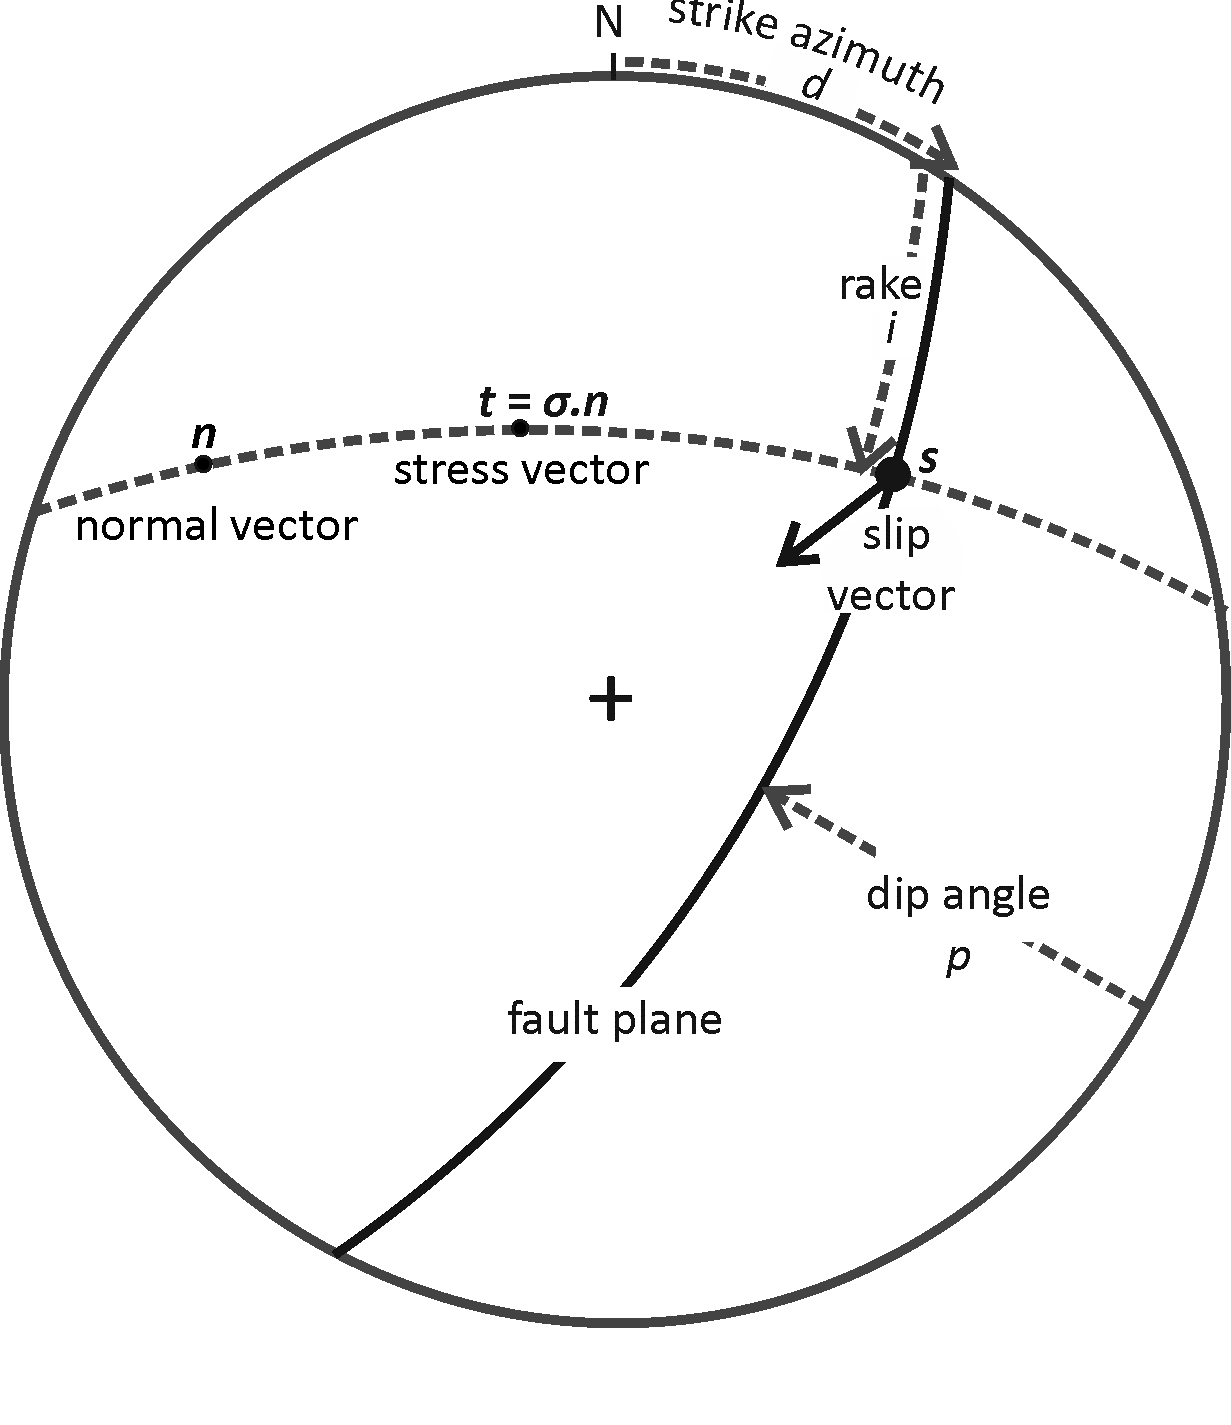
\includegraphics[scale=0.2]{Fig1b}
\caption{Lower hemisphere equal-area projection showing input parameters, $d$, $p$, and $i$, and the stress vectors.}
\label{fig1}
\end{figure}

The normal vector $\bm{n}$ and the slip vector $\bm{s}$ can be expressed in their component form as:
\begin{equation} \label{1}
\begin{split}
n_{x} &= sin(p).cos(d), \\
n_{y} &= -sin(p).sin(d), \\
\text{and}\ n_{z} &= cos(p).    
\end{split}
\end{equation}
\begin{equation} \label{2}
\begin{split}
s_{x} &= cos(i).sin(d) - sin(i).cos(p).cos(d), \\
s_{y} &= cos(i).cos(d) - sin(i).cos(p).sin(d),\\
\text{and}\ s_{z} &= sin(i).sin(p).
\end{split}
\end{equation}

\section{Representation of the Reduced Stress Tensor}
In continuum mechanics, the Cauchy stress tensor, a 3 x 3 symmetric matrix containing six independent parameters, describes the stress acting at a point. We can further reduce this tensor to only four independent variables (Angelier 1994), by eliminating the depth of burial and pore pressure, since it is impossible to estimate them from fault-slip observations (Angelier, 1994). We describe this reduced stress tensor ($\bm{\sigma}$) using three Euler angles ($\alpha$, $\beta$, $\gamma$) (Celerier, 1988; Celerier et al., 2012) and a stress ellipsoid ratio ($\phi$) (Angelier, 1975, 1994). 

\begin{figure}[h]
\centering
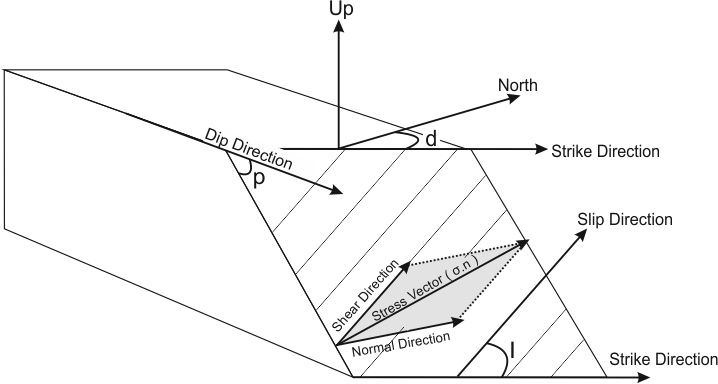
\includegraphics[scale=0.7]{Fig1a}
\caption{Block diagram of a fault surface, showing the normal and shear stress vector components, and the input parameters $d$, $p$, and $i$.}
\label{fig2}
\end{figure}

A symmetric Cauchy stress tensor is given as$-$
\[ 
\begin{bmatrix}
\sigma_{xx} & \sigma_{xy} & \sigma_{xz}\\
\sigma_{xy} & \sigma_{yy} & \sigma_{yz}\\
\sigma_{xz} & \sigma_{yz} & \sigma_{zz}
\end{bmatrix}.
\]
Here, the components along the main diagonal are the eigenvectors of the matrix, which are mutually perpendicular, and the corresponding eigenvalues are called principal stresses. The principal stresses are hereafter referred to as $\sigma_{1}, \sigma_{2}$ and $\sigma_{3}$ in the decreasing order of their magnitudes. The rest of the non diagonal components are called the shear stresses. The shear stresses will vanish in a principal stress frame of reference. Therefore, if we rotate this stress tensor into a principal stress frame, we get the principal stress tensor $ ( \bm{\sigma_{p}} ) - $

\begin{equation}
\label{3}
\bm{\sigma_{p}} =  
\begin{bmatrix}
\sigma_{1} & 0 & 0\\
0 & \sigma_{2} & 0\\
0 & 0 & \sigma_{3}
\end{bmatrix}.
\end{equation}
It is important to note that we cannot completely determine all the values of these principal stresses from fault-slip observations. This is because it is impossible to determine the pore fluid pressure and the depth of burial, unless additional information about friction is given, and because the slip directions are virtually insensitive to these parameters. But we can determine the relative magnitudes of the three principal stresses, and the orientation of these stresses. This parameter $\phi$, called the stress ellipsoid ratio, gives us the shape of the stress ellipsoid (An ellipsoid with the three axes as the principal stress magnitudes).

If we add an isotropic stress tensor $-\sigma_{3}\bm{I}$ (where $\bm{I}$ is the identity matrix) to Eq. \ref{3}, and then multiply the equation with $\frac{1}{\sigma_{1} - \sigma_{3}}$, then we get a reduced stress tensor$(\bm{\sigma_{0}})$ in the principal stress reference frame, given by: 

\begin{equation} \label{4}
\bm{\sigma_{0}} =  
\begin{bmatrix}
1 & 0 & 0\\
0 & \phi & 0\\
0 & 0 & 0
\end{bmatrix},
\end{equation}
and
\begin{equation}
\label{5}
\phi = \frac{ \sigma_{2} - \sigma_{3} }{ \sigma_{1} - \sigma_{3} }.
\end{equation}
  
This tensor can then be rotated to align along the geographic coordinate system, in which the fault geometry is measured. This rotation is described by the Euler angles $\alpha, \beta$ and $\gamma$ (Celerier 1988, Yamaji 2000).

The composite rotation matrix $\bm{R}$ can be written as:
\small
\noindent
\begin{equation} \label{6}
\bm{R} =
\left[
\begin{smallmatrix}
sin(\alpha)sin(\beta) & cos(\alpha)cos(\gamma)-sin(\alpha)cos(\beta)sin(\gamma) & -cos(\alpha)sin(\gamma)-sin(\alpha)cos(\beta)cos(\gamma)\\
-cos(\alpha)sin(\beta) & sin(\alpha)cos(\gamma)+cos(\alpha)cos(\beta)sin(\gamma) & -sin(\alpha)sin(\gamma)+cos(\alpha)cos(\beta)cos(\gamma)\\
cos(\beta) & sin(\beta)sin(\gamma) & sin(\beta)cos(\gamma)
\end{smallmatrix} \right].
\end{equation}

\normalsize
Restricting the maximum principal stress axis to the upper half sphere, we can obtain the ranges of values of the Euler angles as follows (Celerier 1988, 2012) $-$
\begin{equation}
\label{7}
0 \le \alpha < 2\pi; \hspace{3mm} 0 \le \beta \le \frac{\pi}{2}; \hspace{3mm} 0 \le \gamma < 2\pi. \hspace{3mm}
\end{equation} 
Also, from equation \ref{5}, we can deduce that that the range of values of $\phi$ is $-$
\begin{equation}
\label{8}
0 \le \phi \le 1.
\end{equation}
The reduced stress tensor after rotation ($\bm{\sigma}$) can be expressed in terms of ($\bm{\sigma_{0}}$) and the rotation matrix ($\bm{R}$) as-
\begin{equation} \label{9}
\bm{\sigma} = \bm{R}.\bm{\sigma_{0}}.\bm{R^T}.
\end{equation}
Thus, we have a total of four independent variables: the three Euler angles $(\alpha, \beta, \gamma)$ and the stress ellipsoid ratio $(\phi)$ as our output parameters which completely describe the stress tensor  ($\bm{\sigma}$), to be estimated using inversion technique. 

\section{Mechanism of Fault-Slip}
Mohr Coulomb criteria , and adequately explains failure along intact rocks. But it is often seen that the rock masses have a preferred weakness plane, along which they tend to slip. Furthermore, a majority of faults slip along pre-existing fault planes. These pre-existing faults along with faults in anisotropic materials are referred to as reactivated faults. The mechanism of reactivated faults was given by Wallace (1951) and Bott(1959).

Wallace (1951) suggested that the slip in faults occur along the direction and orientation of maximum shear stress. Bott (1959) derived the equations for the same by considering the stress vector acting on different fault planes with variable orientations. This Wallace-Bott hypothesis is also able to explain oblique slip faulting, and hence can be used for non Andersonian stress states as well.

The traction vector ($\bm{T}$) on a fault plane with normal ($\bm{n}$) in terms of the Cauchy stress tensor ($\bm{\sigma}$) is given as (Fig. \ref{fig2}) - 
\begin{equation}
\label{10}
\bm{T} = \bm{\sigma}.\bm{n}.
\end{equation}
The normal and tangential components of this vector (Fig. \ref{fig2}) are the normal and shear traction vectors ($\bm{\sigma_{n}}$ and $\bm{\sigma_{s}}$), given by $-$
\begin{align}
\label{11}
\bm{\sigma_{n}} &= (\bm{n} . \bm{T}) \bm{n} = (\bm{n} . (\bm{\sigma}.\bm{n}))\bm{n},\\
\label{eq:15}
\bm{\sigma_{s}} &= \bm{T} - \bm{\sigma_{n}} = \bm{\sigma}.\bm{n} - (\bm{n} . (\bm{\sigma}.\bm{n}))\bm{n}.
\end{align}
The Wallace-Bott Hypothesis says that this shear stress direction is coincident with the direction of slip, $\bm{s}$, defined in Section \ref{sec:2.1}. Therefore, in terms of $\bm{s}$, the shear stress vector is $-$
\begin{equation}
\label{13}
\bm{\sigma_{s}} = (\bm{s} . \bm{T})\bm{s} = (\bm{s} . (\bm{\sigma}.\bm{n}))\bm{s}.
\end{equation}

\section{The Mean Misfit Function}
The objective function to be minimized for the stress tensor is the sum of misfits between the observed slip direction and the shear component of stress vector (Yamaji 2007). The misfit function is a measure of how well an individual model set satisfies the given set of observations. The misfit angle, $M$, between the two unit vectors ($\bm{\sigma_{s}}/|\bm{\sigma_{s}}|$ and $\bm{s}$) is defined as:

\begin{equation} \label{14}
M = \left|tan^{-1} \left(\frac{|  (\bm{\sigma_{s}}/|\bm{\sigma_{s}}|) \times \bm{s}|}{ (\bm{\sigma_{s}}/|\bm{\sigma_{s}}|) \cdot \bm{s}}\right)\right|.
\end{equation}  

Angelier (1975) suggested the following misfit function for minimization-

\begin{equation} \label{15}
G = sin\left(\frac{M}{2}\right),
\end{equation} 
where $0 \le M < 2\pi$. This function minimizes the angular misfit between the two vectors, the observed slip direction and the predicted direction of maximum shear stress.

Another minimization function, which minimizes the misfit between the magnitudes of shear components, is (Angelier et al., 1982):

\begin{equation} \label{16}
H = \left| \bm{s} . (\bm{\sigma}.\bm{n}) - \sqrt{( (\bm{\sigma}.\bm{n})^2 - (\bm{n} . (\bm{\sigma}.\bm{n}))^2 )} \right|.
\end{equation}

We define a misfit function, $F$, that accounts for both, the angular misfit $G$ and the magnitude misfit of the shear component $H$, as:

\begin{equation} \label{17}
F = \lambda G + (1-\lambda) H,
\end{equation}
where $\lambda$ is the weighting parameter in the range $0 \le \lambda \le 1$. A similar function is described by Delvaux and Sperner (2003).The mean misfit function $\bar{F}$, is average of the $F$ for all the faults in a given population, and this function is minimized for determination of the reduced stress tensor.